\documentclass[dvipdfmx]{standalone}
\usepackage{tikz}
\usepackage{amsmath}
\usepackage{amssymb}
\usepackage{amsfonts}
\usepackage{graphicx}
\usepackage{float}
\usepackage{xcolor}
\usetikzlibrary{shapes.geometric, arrows, calc}

\definecolor{decisionColor}{HTML}{BFE4FF}
\tikzstyle{decision} = [diamond, 
aspect=2.5,
font=\large,
minimum width=3cm,
minimum height=2cm, 
text centered,
rounded corners,
fill=decisionColor]

\tikzstyle{endNode} = [rectangle,
rounded corners,
align=center,
font=\large,
minimum width=3.5cm,
minimum height=2cm,
text centered,
fill=blue!30!white]

\newcommand{\DrawZigzagArrow}[4][]{%
  \draw[->, rounded corners, #1] (#2) -- ($ (#2)!0.5!(#2|-#3) $) -- ($ (#3)!0.5!(#3|-#2) $) -- (#3);
  \ifnum#4=1
    \node[circle,fill=green!30!white] at ($ (#2)!0.5!(#3) $) {Yes}
  \else
    \node[circle,fill=red!30!white] at ($ (#2)!0.5!(#3) $) {No}
  \fi
}
\begin{document}

\begin{tikzpicture}
  \node[anchor=north,decision] (dec1) at (+0,+0) {$\mathrm{dom}~f = \mathbb{R}^n$か?};
  \node[anchor=north,decision] (dec2) at (+3,-3.5) {閉凸関数か?};
  \node[anchor=north,decision] (dec3) at (+0,-7) {1変数関数か?};
  \node[anchor=north,endNode]  (end1) at (-3,-3.5) {連続\\$ax+b,x^2,|x|,e^x$など};
  \node[anchor=north,endNode]  (end2) at (+6,-7) {様々あり得る\\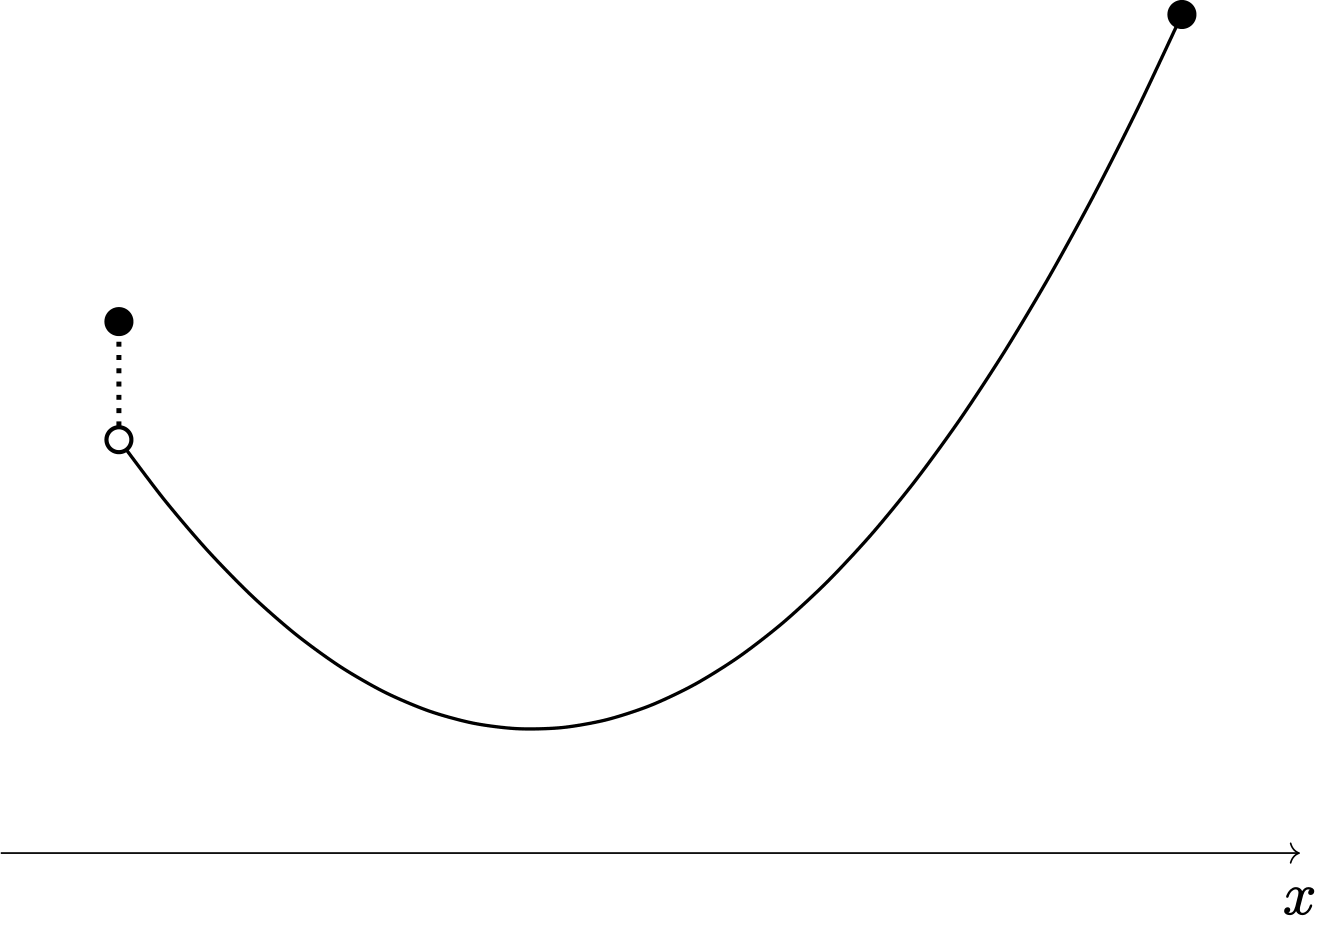
\includegraphics[width=3.2cm]{../figs/closed_interval.png}};
  \node[anchor=north,endNode]  (end3) at (-3,-10.5) {連続\\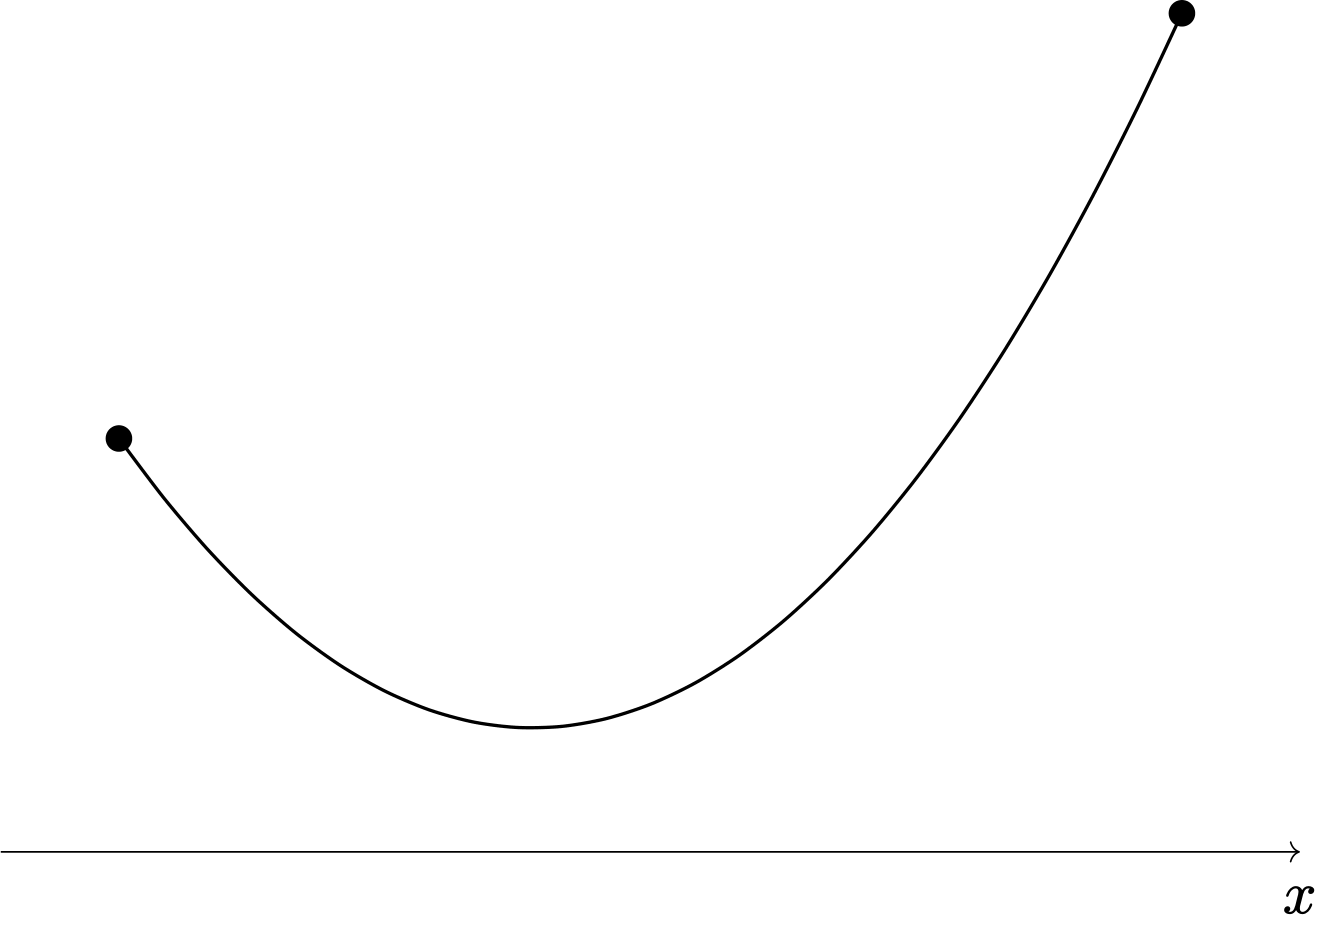
\includegraphics[width=3.2cm]{../figs/closed_interval_closed_convex.png}};
  \node[anchor=north,endNode]  (end4) at (+3,-10.5) {下半連続だが\\連続とは限らない\\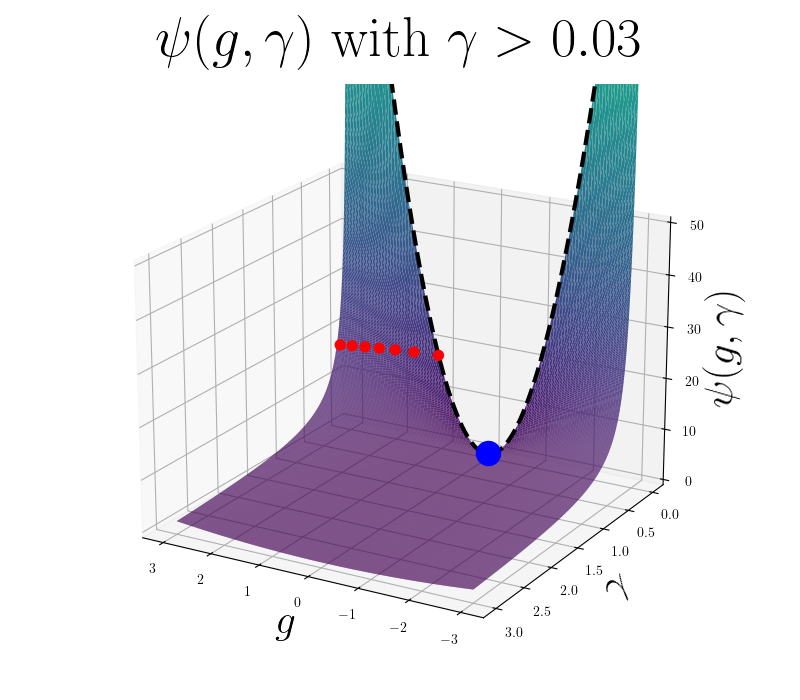
\includegraphics[width=3.2cm]{../psi/psi_0.03.png}};

  \DrawZigzagArrow[thick,>=stealth]{dec1.south}{end1.north}{1};
  \DrawZigzagArrow[thick,>=stealth]{dec1.south}{dec2.north}{0};
  \DrawZigzagArrow[thick,>=stealth]{dec2.south}{dec3.north}{1};
  \DrawZigzagArrow[thick,>=stealth]{dec2.south}{end2.north}{0};
  \DrawZigzagArrow[thick,>=stealth]{dec3.south}{end3.north}{1};
  \DrawZigzagArrow[thick,>=stealth]{dec3.south}{end4.north}{0};

  \node[rounded corners,align=center,draw,font=\Large] at (+5.5,-1.75) {凸関数$f$\\$(\mathrm{dom}~f \neq \emptyset)$};
\end{tikzpicture}
\end{document}